%%%%%%%%%%%%%%%%%%%%%%%%%%%%%%%%%%%
%This is the LaTeX ARTICLE template for RSC journals
%Copyright The Royal Society of Chemistry 2016
%%%%%%%%%%%%%%%%%%%%%%%%%%%%%%%%%%%

\documentclass[twoside,twocolumn,9pt]{article}

\usepackage{tgheros}
\renewcommand{\familydefault}{\sfdefault}

\usepackage{extsizes}
\usepackage[super,sort&compress,comma]{natbib} 
\usepackage[version=3]{mhchem}
\usepackage[left=1.5cm, right=1.5cm, top=1.785cm, bottom=2.0cm]{geometry}
\usepackage{balance}
\usepackage{mathptmx}
\usepackage{sectsty}
\usepackage{graphicx} 
\usepackage{lastpage}
\usepackage[format=plain,justification=justified,singlelinecheck=false,font={stretch=1.125,small,sf},labelfont=bf,labelsep=space]{caption}
\usepackage{float}
\usepackage{fancyhdr}
\usepackage{fnpos}
\usepackage[english]{babel}
\addto{\captionsenglish}{%
  \renewcommand{\refname}{Notes and references}
}
\usepackage{array}
\usepackage{droidsans}
\usepackage{charter}
\usepackage[T1]{fontenc}
\usepackage[usenames,dvipsnames]{xcolor}
\usepackage{setspace}
\usepackage[compact]{titlesec}
\usepackage[utf8]{inputenc}
%%%Please don't disable any packages in the preamble, as this may cause the template to display incorrectly.%%%

\usepackage{xcolor}
\definecolor{ugent_blue}{RGB}{30, 100, 200}
\definecolor{ugent_yellow}{cmyk}{.0, .10, 1, 0}

\usepackage{titlesec}
\titleformat{\section}
{\color{ugent_blue}\normalfont\Large\bfseries}
{\color{ugent_blue}\thesection}{1em}{}

\usepackage[colorlinks=true,linkcolor=black,citecolor=ugent_blue]{hyperref}

\usepackage{lineno}
\linenumbers

%\AtEveryCite{\color{ugent_blue}}



\usepackage{epstopdf}%This line makes .eps figures into .pdf - please comment out if not required.

\definecolor{cream}{RGB}{222,217,201}

\begin{document}

\pagestyle{fancy}
\thispagestyle{plain}
\fancypagestyle{plain}{
%%%HEADER%%%
\renewcommand{\headrulewidth}{0pt}
}
%%%END OF HEADER%%%

%%%PAGE SETUP - Please do not change any commands within this section%%%
\makeFNbottom
\makeatletter
\renewcommand\LARGE{\@setfontsize\LARGE{15pt}{17}}
\renewcommand\Large{\@setfontsize\Large{12pt}{14}}
\renewcommand\large{\@setfontsize\large{10pt}{12}}
\renewcommand\footnotesize{\@setfontsize\footnotesize{7pt}{10}}
\makeatother

\renewcommand{\thefootnote}{\fnsymbol{footnote}}
\renewcommand\footnoterule{\vspace*{1pt}% 
\color{cream}\hrule width 3.5in height 0.4pt \color{black}\vspace*{5pt}} 
\setcounter{secnumdepth}{5}

\makeatletter 
\renewcommand\@biblabel[1]{#1}            
\renewcommand\@makefntext[1]% 
{\noindent\makebox[0pt][r]{\@thefnmark\,}#1}
\makeatother 
\renewcommand{\figurename}{\small{Fig.}~}
\sectionfont{\sffamily\Large}
\subsectionfont{\normalsize}
\subsubsectionfont{\bf}
\setstretch{1.125} %In particular, please do not alter this line.
\setlength{\skip\footins}{0.8cm}
\setlength{\footnotesep}{0.25cm}
\setlength{\jot}{10pt}
\titlespacing*{\section}{0pt}{4pt}{4pt}
\titlespacing*{\subsection}{0pt}{15pt}{1pt}
%%%END OF PAGE SETUP%%%

%%%FOOTER%%%
\fancyfoot{}
\fancyfoot[LO,RE]{\vspace{-7.1pt}\includegraphics[height=9pt]{head_foot/LF}}
\fancyfoot[CO]{\vspace{-7.1pt}\hspace{11.9cm}\includegraphics{head_foot/RF}}
\fancyfoot[CE]{\vspace{-7.2pt}\hspace{-13.2cm}\includegraphics{head_foot/RF}}
\fancyfoot[RO]{\footnotesize{\sffamily{1--\pageref{LastPage} {\color{ugent_yellow} ~\textbar } \hspace{2pt}\thepage}}}
\fancyfoot[LE]{\footnotesize{\sffamily{\thepage~{\color{ugent_yellow} ~\textbar }\hspace{4.65cm} 1--\pageref{LastPage}}}}
\fancyhead{}
\renewcommand{\headrulewidth}{0pt} 
\renewcommand{\footrulewidth}{0pt}
\setlength{\arrayrulewidth}{1pt}
\setlength{\columnsep}{6.5mm}
\setlength\bibsep{1pt}
%%%END OF FOOTER%%%

%%%FIGURE SETUP - please do not change any commands within this section%%%
\makeatletter 
\newlength{\figrulesep} 
\setlength{\figrulesep}{0.5\textfloatsep} 

\newcommand{\topfigrule}{\vspace*{-1pt}% 
\noindent{\color{cream}\rule[-\figrulesep]{\columnwidth}{1.5pt}} }

\newcommand{\botfigrule}{\vspace*{-2pt}% 
\noindent{\color{cream}\rule[\figrulesep]{\columnwidth}{1.5pt}} }

\newcommand{\dblfigrule}{\vspace*{-1pt}% 
\noindent{\color{cream}\rule[-\figrulesep]{\textwidth}{1.5pt}} }

\makeatother
%%%END OF FIGURE SETUP%%%

%%%TITLE, AUTHORS AND ABSTRACT%%%
\twocolumn[
  \begin{@twocolumnfalse}
{\includegraphics[height=30pt]{head_foot/journal_name}\hfill\raisebox{0pt}[0pt][0pt]{\includegraphics[height=55pt]{head_foot/RSC_LOGO_CMYK}}\\[1ex]
\includegraphics[width=18.5cm]{head_foot/header_bar}}\par
\vspace{1em}
\sffamily
\begin{tabular}{m{4.5cm} p{13.5cm} }

& \noindent\LARGE{\textbf{Orbital optimisation for Richardson-Gaudin wavefunctions$^\dag$}} \\%Article title goes here instead of the text "This is the title"
\vspace{0.3cm} & \vspace{0.3cm} \\

& \noindent\large{Charles-Émile Fecteau\textit{$^{a,b}$}, Guillaume Acke\textit{$^{a}$}, Patrick Bultinck\textit{$^{a}$} and Paul A. Johnson\textit{$^{b}$}} \\%Author names go here instead of "Full name", etc.

& \\

& \noindent\normalsize{Do \emph{not} write an abstract. That will be done when the outline has matured into a completed paper.} \\%The abstrast goes here instead of the text "The abstract should be..."

\end{tabular}

\end{@twocolumnfalse} \vspace{1.6cm}]
%%%END OF TITLE, AUTHORS AND ABSTRACT%%%

%%%FONT SETUP - please do not change any commands within this section
\renewcommand*\rmdefault{bch}\normalfont\upshape
\rmfamily
\section*{}
\vspace{-1cm}

% %%%FOOTNOTES%%%

\footnotetext{\textit{$^{a}$~Department of Chemistry, Ghent University, Krijgslaan 281 (S3), B-9000 Ghent, Belgium}}
\footnotetext{\textit{$^{b}$~Department of Chemistry, Université laval, 2325 rue de l'Université, Québec, Canada, G1V 0A6}}

% %Please use \dag to cite the ESI in the main text of the article.
% %If you article does not have ESI please remove the the \dag symbol from the title and the footnotetext below.
% \footnotetext{\dag~Electronic Supplementary Information (ESI) available: [details of any supplementary information available should be included here]. See DOI: 00.0000/00000000.}
% %additional addresses can be cited as above using the lower-case letters, c, d, e... If all authors are from the same address, no letter is required

% \footnotetext{\ddag~Additional footnotes to the title and authors can be included \textit{e.g.}\ `Present address:' or `These authors contributed equally to this work' as above using the symbols: \ddag, \textsection, and \P. Please place the appropriate symbol next to the author's name and include a \texttt{\textbackslash footnotetext} entry in the the correct place in the list.}

%%%END OF FOOTNOTES%%%

%%%MAIN TEXT%%%%

\section{Introduction}

Orbital-optimised doubly-occupied configuration interaction (OO-DOCI) computations yield the most precise result one can expect to obtain through a geminal approach with a given orbital basis set. In other words, for a given set of orbitals, this approach gives the exact solution to the seniority-zero coulomb Hamiltonian. Incidently, its optimised orbitals are also the optimal orbitals for any geminal-based approach.

This makes this method an very useful reference tool as we develop a variationnal Richardson-Gaudin (varRG) approach based on wavefunction ansatz made from products of Richardson-Gaudin geminals\cite{Johnson:2}\cite{Fecteau:2}
, both as a source for the optimal orbitals (until we develop an independent orbital-optimisation routine) and as a comparison standard for the precision we can hope to achieve.

It is therefore relevant to compute OO-DOCI dissociation curves for various small systems as a reference point. We are notably interested in the following systems, for the STO-6G and cc-pVDZ orbital basis :

\begin{itemize}
    \item Hydrogen polymer chains : $H_4$, $H_6$ and $H_8$ 
    \item Homonuclear diatomics : $He_2$, $Li_2$, $Be_2$, $B_2$, $C_2$, $N_2$, $O_2$, $F_2$ and $Ne_2$ (cc-pVDZ only)
    \item 12-electron diatomics : 
    $LiF$, $BeO$, $BN$, $CN^+$ and $CO^{2+}$ (and $C_2$)
    \item 14-electron diatomics : 
    $CN^-$, $CO$, $NO^+$ and $O_2^{2+}$ (and $N_2$)
\end{itemize}

%\section{Theory}

\section{Results and discussion}
\subsection{STO-6G}
\subsubsection{Hydrogen polymer chains}
All hydrogen polymer chains dissociation curves were easily computed and yielded smooth results. 

%INSERT FIGURES

\subsubsection{Homonuclear diatomics}
$Li_2$, $N_2$, $O_2$ and $F_2$ dissociations curves were relatively easily computed to obtain smooth results. For the larger systems ($N_2$, $O_2$ and $F_2$), some points yielded results that layed outside the curve; however, it was possible to recompute those points to get adequate results, thus these invalid results were attributed to bad convergence of the optimisation algorithm (CMA-ES, which has a stochastic nature).

%INSERT FIGURES

The curves for $Be_2$ and $C_2$, however, consistently produced unexpected shoulders between the minimum and dissociation (see figures \ref{Be2_bad} and \ref{C2_bad}), whereas $B_2$ shows an unphysical double well (see figure \ref{B2_bad}).

\begin{figure}[h]
  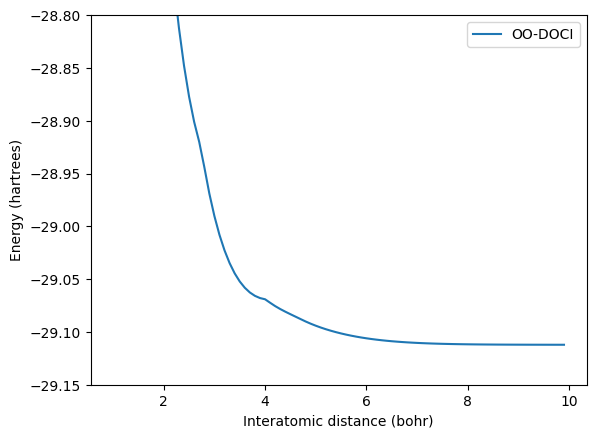
\includegraphics[width=\linewidth]{Be2.png}
  \caption{OO-DOCI dissociation curve of $Be_2$ in the STO-6G orbital basis}\label{Be2_bad}
\end{figure}

\begin{figure}[h]
  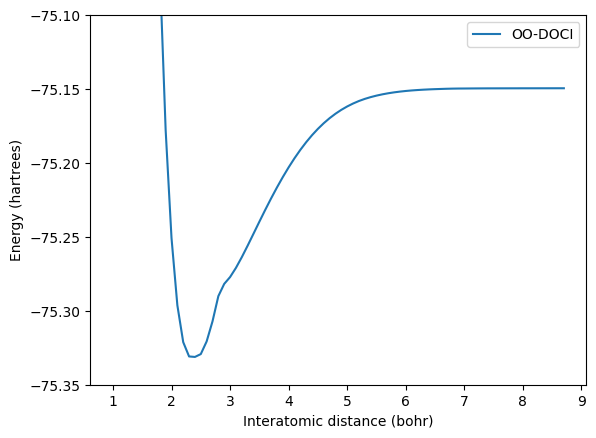
\includegraphics[width=\linewidth]{C2.png}
  \caption{OO-DOCI dissociation curve of $C_2$ in the STO-6G orbital basis}\label{C2_bad}
\end{figure}

\begin{figure}[h]
  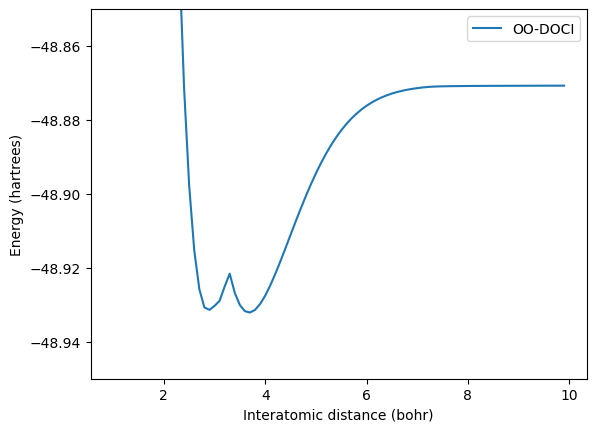
\includegraphics[width=\linewidth]{B2.png}
  \caption{OO-DOCI dissociation curve of $B_2$ in the STO-6G orbital basis}\label{B2_bad}
\end{figure}

Various alternatives for the initial guess for the orbitals have been used (with $B_2$ and $C_2$ specifically) to obtain better results :

\begin{itemize}
  \item Points were computed reusing the orbital rotation of the previous point in the curve, approaching from both the right and the left.
  \item Computations were done using DFT orbitals as an initial guess (using b3lyp, lda, pbe and pw91 functionals).
  \item Computations were done using CISD natural orbitals as an initial guess.
\end{itemize}

Unfortunately, non of these approaches helped in obtaining better dissociation curves, instead they all converged on the same results as the initial brute-force approach. 

\subsubsection{12-electron diatomics}

Similarly to some of the homonuclear diatomics mentioned, all 12-electron dissociation curves present unexpected shoulders. The same approaches that had been attempted for $B_2$ and $C_2$ have been used with $B_N$ as well, to no avail.

\begin{figure}[h]
  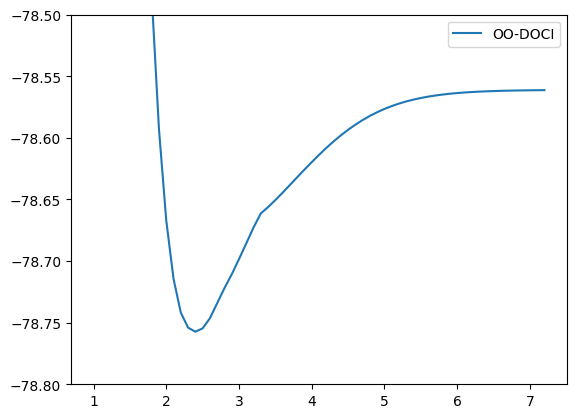
\includegraphics[width=\linewidth]{BN.png}
  \caption{OO-DOCI dissociation curve of $BN$ in the STO-6G orbital basis}\label{BN_bad}
\end{figure}

%INSERT FIGURES

\subsubsection{14-electron diatomics}

Like for 12-electron systems, most 14-electron dissociation curves present unexpected shoulders. The one exception is $CN^-$, which yielded a smooth curve.

%INSERT FIGURES

\subsection{cc-pVDZ}
\subsubsection{Hydrogen polymer chains}
Computations underway.

\subsubsection{Homonuclear diatomics}
Computations underway.

\subsubsection{12-electron diatomics}
Computations underway.

\subsubsection{14-electron diatomics}
Computations underway.

One issue that arises when computing these dissociation curves (as well as those for $N_2$, $O_2$, $F_2$ and $Ne_2$) is that the maximal computation time allowed on some compute canada clusters is 7 days, but the computation of even a single point for systems with 14 electrons or more in the cc-pVDZ orbital basis takes more time than that. The cluster cedar allows for longer computations, but if the possibility of segmenting CMA-ES optimisation for a single point should be investigated and implemented if possible. 

\section{Conclusions}

\section{Acknowledgements}

\section{Appendix}

%%%END OF MAIN TEXT%%%

%The \balance command can be used to balance the columns on the final page if desired. It should be placed anywhere within the first column of the last page.

\balance

%If notes are included in your references you can change the title from 'References' to 'Notes and references' using the following command:
%\renewcommand\refname{Notes and references}

%%%REFERENCES%%%
\bibliography{outline} %You need to replace "rsc" on this line with the name of your .bib file
\bibliographystyle{aip} %the AIP's .bst file

\end{document}